% BEGIN TEMPLATE
\documentclass{article}
\usepackage{graphicx}
\usepackage{hyperref} 
\usepackage{xcolor}
\usepackage{nameref}
\usepackage{listings}
\usepackage{float}
\usepackage[title]{appendix}
\graphicspath{ {../../images/} }
\bibliographystyle{acm}
% CHANGE THESE
\newcommand{\courseListing}{CSCI 8110-001}
\newcommand{\courseName}{Advanced Machine Learning Applications}
\newcommand{\assignmentTitle}{Homework Assignment \#1}
\newcommand{\assignmentSubtitle}{Convolutional Autoencoders}

\hypersetup{
    colorlinks,
    linkcolor={red!50!black},
    citecolor={blue!50!black},
    urlcolor={blue!80!black}
}
\urlstyle{same}
\definecolor{codegreen}{rgb}{0,0.6,0}
\definecolor{codegray}{rgb}{0.5,0.5,0.5}
\definecolor{codepurple}{rgb}{0.58,0,0.82}
\lstdefinestyle{mystyle}{
    commentstyle=\color{codegreen},
    keywordstyle=\color{magenta},
    numberstyle=\tiny\color{codegray},
    stringstyle=\color{codepurple},
    basicstyle=\ttfamily\footnotesize,
    breakatwhitespace=false,         
    breaklines=true,                 
    captionpos=b,                    
    keepspaces=true,                 
    numbers=left,                    
    numbersep=5pt,                  
    showspaces=false,                
    showstringspaces=false,
    showtabs=false,                  
    tabsize=2
}

\lstset{style=mystyle}

\begin{document}
  \begin{center}
  
\includegraphics[scale=0.15]{UNO-Logo-Color.png}
  \\[0.3in]
  \textbf{\courseListing{}}\\
  \courseName{}
  \\[0.75in]
  \textbf{\assignmentTitle{}}\\
  \assignmentSubtitle{}
  \\[0.75in]
  \textbf{Patrick Davlin}
  \\[0.75in]
  \textbf{Computer Science Department}\\
  \textbf{Peter Kiewit Institute}\\
  \textbf{University of Nebraska}
  \\[0.75in]
  \textbf{Fall 2020}
  \\[0.3in]
  
\includegraphics[scale=0.075]{UNO-Icon-Color.png}
  \newpage
\end{center}
  \graphicspath{{./images/}}
% END TEMPLATE

\section{Project Setup}
\par All work in this project was developed and executed using the Paperspace Gradient service.
Gradient allows for rapid setup of TensorFlow notebooks on GPU-powered machines, which was ideal for this first project given that optimizing a personal computer for running machine learning models proved difficult at the outset.
The downside, however, is that without a more expensive subscription, Gradient only allows for six hours' worth of compute time at once (further discussed in \nameref{procresults}).
This limits the amount of time that computations can run, and Gradient is strict about cutting off at that point--more than one computation for this project was cut off due to poor calculation of the time a task would take to complete.

\par Once the Gradient instance is up and running, the instance is a reasonably straightforward Jupyter Notebook running TensorFlow 2.0.
Blocks of code can be executed interactively and accessed over the web.
A static version of the notebook can be accessed by clicking on \href{https://console.paperspace.com/te7vzjiu3/notebook/prz0iko1d}{this link}.

\section{Process \& Results} \label{procresults}
\par Procedurally, this assignment had a very straightforward premise: implement a convolutional autoencoder, with a reuse of the structure outlined in lecture allowed.

\par Initially, the given task proved difficult for two reasons. 
First, with minimal experience in setting up Jupyter notebooks or working with TensorFlow/Keras, it was challenging to set up and successfully run code out of the gate in the Paperspace instance.
Some time needed to be spent learning about some of the conventions of working with Jupyter notebook files to ensure that proper conventions were being followed.

\par The second, more project-specific, issue was that adapting the code from class to accept an input size appropriate to the CIFAR-10 dataset was not immediately intuitive.
Partly because of the three color channels in the data (as opposed to one) and the size of the kernels used (3x3), the expected input was initially set to a shape of (28,28,1), where the image inputs were each of the shape (32,32,3).
This was a byproduct of inexperience with TensorFlow and, initially, a lack of understanding of how the shape of an input changes as the result of convolution steps. 
The remedy was relatively simple, though: on each step where \lstinline[language=Python]{Conv2D()} was used, it was important to add the \lstinline[language=Python]{padding='same'} parameter so that the extra pixels at the end of each image weren't omitted.

\par Having solved these issues, the intent and process of the assignment became more clear.
Code provided in the lecure materials had several pre-defined convolutional layers that were re-implemented as shown below:
\begin{lstlisting}[language=Python]
x = Conv2D(16, (3, 3), 
    activation='relu', padding='same')(input_img)
x = MaxPooling2D((2, 2), padding='same')(x)
x = Conv2D(8, (3, 3), activation='relu', padding='same')(x)
x = MaxPooling2D((2, 2), padding='same')(x)
x = Conv2D(8, (3, 3), activation='relu', padding='same')(x)
encoded = MaxPooling2D((2, 2), padding='same')(x)

x = Conv2D(8, (3, 3), activation='relu', padding='same')(encoded)
x = UpSampling2D((2, 2))(x)
x = Conv2D(8, (3, 3), activation='relu', padding='same')(x)
x = UpSampling2D((2, 2))(x)
x = Conv2D(16, (3, 3), activation='relu', padding='same')(x)
x = UpSampling2D((2, 2))(x)
decoded = 
    Conv2D(3, (3, 3), activation='sigmoid', padding='same')(x)
\end{lstlisting}

\par The Keras model was then fit against the test Cifar10 data as follows:

\begin{lstlisting}[language=Python]
autoencoder.fit(x_train, x_train, 
                epochs=50,
                batch_size=256,
                shuffle=True,
                validation_data=(x_test, x_test))

\end{lstlisting}

\par Using this model, each input image was first encoded and then decoded through the convolution and max pooling layers.
The input and output images can be compared in \autoref{fig:initial}:

\begin{figure}[H]
    \centering
    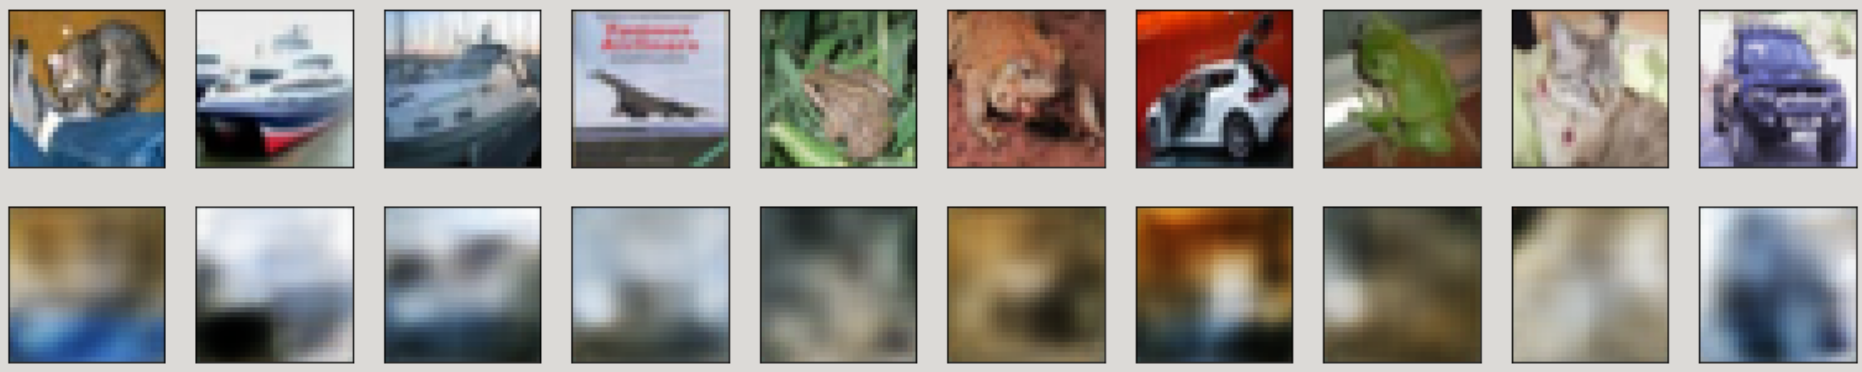
\includegraphics[width=4.75in]{csci-8110/hw-1/hw1-images/16-8-8-50.png}
    \caption{CAE with layer values 16/8/8, with 50 training epochs}
    \label{fig:initial}
\end{figure}

\par \autoref{fig:initial} represents a good start, given that the model can clearly output a decoded set of images, but the outcome is not a visually clear result. 
Fortunately, it was clear at this point that there are three "knobs" that can be adjusted in order to further enhance the autoencoder's output:
\begin{enumerate}
  \item \textit{The number of filters in each layer}, the number in the first argument of the \lstinline[language=Python]{Conv2D()} function, to increase the resolution  of processing at each layer;
  \item \textit{The number of epochs}, to increase the size of the training set for the model; and
  \item \textit{The number of layers}, or adding more calls of \lstinline[language=Python]{Conv2D()} and \lstinline[language=Python]{MaxPooling2D()} in the decoding or encoding steps.
\end{enumerate}

\par For this report, the first two options were explored. 
The general strategy when adjusting each of these three parameters was fairly straightforward--making the numbers bigger makes the resulting image set clearer.
It was important to consider the intersection between the complexity of the model and the number of training epochs run.
The instructor-provided model ran each epoch in about 2 seconds, but other versions of the model took seven seconds or more. On the upper end, the most complex model took 40 seconds per epoch, so care had to be taken so that models would be able to run before the Paperspace Gradient's cutoff.
There is also a point where adding additional epochs does not improve the output of the model--for one run, the layers used were all set to 32 and the model was run 5,000 times, but the resulting output was not meaningfully clearer than runs of the same model at 500 or 1,000 times.

\par Another consideration is that the order in which numbers of filters is applied is, evidently, conventionally an increasing format while encoding the inputs \cite{KerasLayers}.
Moreover, for the decoding phase, the order should mirror the encoding phase, so if the filters for each layer are, in order, 8, 16, and 32, then the order of layers in the decoding phase should be 32, 16, and 8.

\par There are several outputs from various parameters included in Appendix \ref{modelouts}, but the most relevant of them is the result from what might be considered the "best" setup encountered while working on the assignment.
That model is reflected by the code implementation in Appendix \ref{codelist}. A combination of more filters per layer and a higher number of epochs was used to create a fairly clear result set, shown below:
\begin{figure}[H]
    \centering
    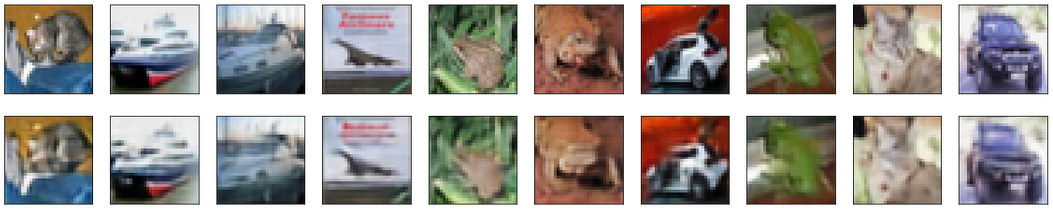
\includegraphics[width=4.75in]{csci-8110/hw-1/hw1-images/64-128-256-500.png}
    \caption{CAE with layer values 64/128/256, with 500 training epochs}
    \label{fig:final}
\end{figure}
\par Of particular note are the fourth image, where the red lines are much more similar than the original image, and the last one, where the rear tire of the truck are most visible.

\par This final model took around an hour to run (7 seconds per epoch $\times$ 500 epochs) and proved to be a fairly reliable middle point between number of epochs and number of filters in layers. 

\section{Conclusions}
As a simple introduction to TensorFlow and Keras, this homework assignment was very informative.
More was learned about implementing and tuning convolutional autoencoders (CAEs) and, generally, some more comfort was developed with using interactive notebooks and TensorFlow commands.
Fortunately, tuning these models was fairly straightforward--so this comfort under the belt is a strong foundation upon which more experience can be built throughout the remainder of the course.

\newpage
\begin{appendices}


\section{Model Output Listing} \label{modelouts}
\begin{figure}[H]
    \centering
    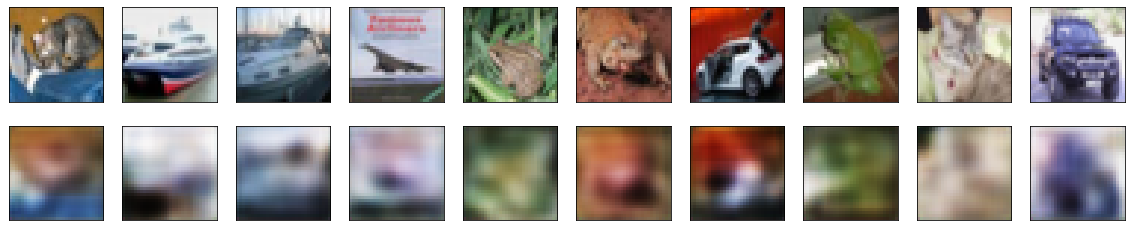
\includegraphics[width=4.75in]{csci-8110/hw-1/hw1-images/8-8-16-50.png}
    \caption{CAE with layer values 8/8/16, with 50 training epochs}
    \label{fig:b1}
\end{figure}
\begin{figure}[H]
    \centering
    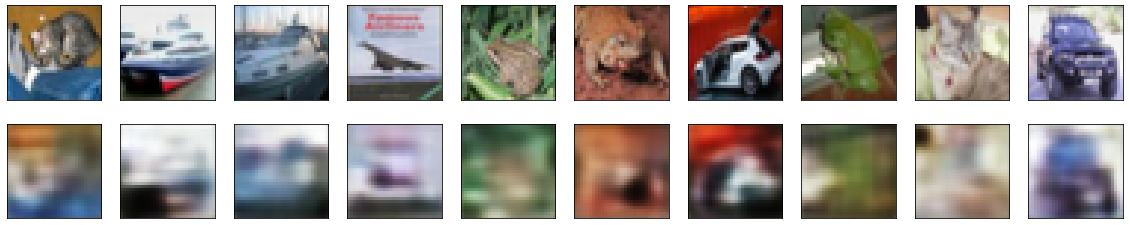
\includegraphics[width=4.75in]{csci-8110/hw-1/hw1-images/8-8-16-250.png}
    \caption{CAE with layer values 8/8/16, with 250 training epochs}
    \label{fig:b2}
\end{figure}
\begin{figure}[H]
    \centering
    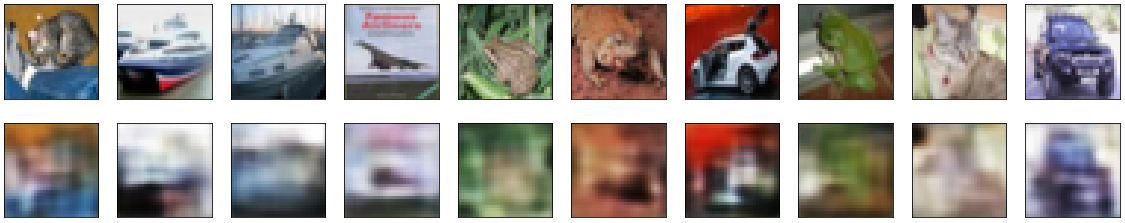
\includegraphics[width=4.75in]{csci-8110/hw-1/hw1-images/8-8-16-1000.png}
    \caption{CAE with layer values 8/8/16, with 1000 training epochs}
    \label{fig:b3}
\end{figure}
\begin{figure}[H]
    \centering
    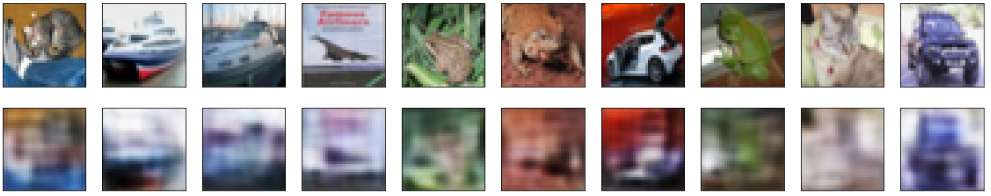
\includegraphics[width=4.75in]{csci-8110/hw-1/hw1-images/8-8-16-5000.png}
    \caption{CAE with layer values 8/8/16, with 5000 training epochs}
    \label{fig:b4}
\end{figure}
\begin{figure}[H]
    \centering
    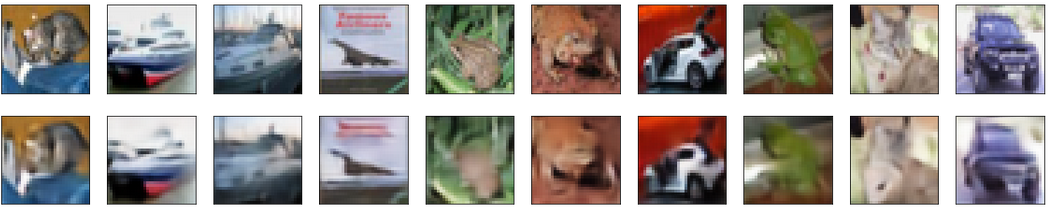
\includegraphics[width=4.75in]{csci-8110/hw-1/hw1-images/256-512-1024-50.png}
    \caption{CAE with layer values 256/512/1024, with 50 training epochs}
    \label{fig:b5}
\end{figure}

\newpage
\section{Complete Code Listing} \label{codelist}
\lstinputlisting[language=Python]{HW1_code.py}
\end{appendices}

\begin{thebibliography}{9}
  \bibitem{KerasLayers} 
  Adrian Rosebrock. 2018. Keras Conv2D and Convolutional Layers. (December 2018). Retrieved September 21, 2020 from https://www.pyimagesearch.com/2018/12/31/keras-conv2d-and-convolutional-layers/.
  
  \end{thebibliography}

\end{document}